\chapter{Experiments}\label{ch:experiments}
In order to find the limits and the usability of the tools in table \ref{table:tools} for high bandwidth session based throughput testing, the tools are subject to various experiments.
The results the research is looking for: 
\begin{itemize}
\item{The capability of generating 40Gb/s of bandwidth.} 
\item{The maximum amount of packets per second.} 
\item{The maximum amount of sessions per second.}
\end{itemize}

The kernel based tools are tested on top of two different kernels. 
FreeBSD 11.0 and Ubuntu 16.04 are used to see if the kernel has any influence on one of the three items stated above.
The reason for using two kernels is that a preliminary test showed major differences in generating UDP packets per second, these differences could also apply for TCP packet generation.  
The DPDK tools are tested on top of the Ubuntu kernel since FreeBSD does not support DPDK.
All experiments described in this chapter are executed in a test environment at Nikhef. The visualization of the test environment is shown in figure \ref{fig:testenv}. \\ 

\begin{figure}[H]
  \includegraphics[scale=0.45]{images/testenv.pdf}
  \caption{Environment used for experiments at Nikhef.}
  \label{fig:testenv}
\end{figure}

The figure shows five server systems, of which three identical servers (A, B and C in table \ref{tab:testmachines}) are used to perform the tests, which results are described in this paper.
During the experiments 2 extra machines (D and E in table 4.1), both containing 100Gb/s Mellanox NIC cards, have been introduced into the network to test links with a capacity up to 100Gb/s to verify if reached limits are resource or hardware based. All servers were connected to a Juniper QFX10002 (device S in Fig. \ref{fig:testenv}), which provides 32 40Gb/s QSFP ports, of which some are configured as a single 100Gb/s interface.

\begin{table}[H]
\centering
\caption{Specifications from the machines used for experiments}
\label{tab:testmachines}
\begin{tabular}{|l|l|l|l|}
\hline
\textbf{Machine} & \textbf{A \& B \& C}                                                                          & \textbf{D}                                                                                    &\textbf{E}                                                                     \\ \hline \hline
Cores / Threads &  2 / 8                                                         &  14 / 56                           & 128 Threads                                                                   \\ \hline
CPU     & \begin{tabular}[c]{@{}l@{}}Intel(R) Xeon(R) CPU \\ E3-1230 v5 @ 3.40GHz\end{tabular} & \begin{tabular}[c]{@{}l@{}}Intel(R) Xeon(R) CPU \\ E5-2697 v3 @ 2.60GHz\end{tabular} & POWER8E                                                               \\ \hline
Memory  & 4x 16GB @ 2133 Mhz                                                                   & 24x 8GB @ 1067Mhz                                                                    & 2x 64GB                                                          \\ \hline
NIC     & \begin{tabular}[c]{@{}l@{}}Intel XL710 \\ 40Gb/s\end{tabular}                        & \begin{tabular}[c]{@{}l@{}}Mellanox ConnectX-4\\ 100Gb/s\end{tabular}                & \begin{tabular}[c]{@{}l@{}}Mellanox ConnectX-4\\ 100Gb/s\end{tabular} \\ \hline
\end{tabular}
\end{table}

Device A is always acting as the destination for traffic unless stated otherwise. Depending on the tests the source can be machine B, C or B and C together.
This depends on the capability of the tools tested at that moment.
For testing beyond 40Gb/s, one of the 100Gb/s machines (D or E) can be used.
Machine M is a Simple Network Management Protocol (SNMP) collector. This SNMP collector queries the test servers every 10 seconds for status. 
Packets per second and bits per second are retrieved from the devices under test.
Switch S is also added to the collector as a data source. 
SNMP is active on the management interface of the devices.
The high bandwidth interfaces are able to connect to each other over a non-routed VLAN. This makes sure the test traffic cannot interfere with SNMP reads from collector M. 

\section{Standards and best practices}\label{sub:rfc}
Multiple RFCs have been written that provide guidelines for throughput testing.
This research refers to RFCs that contain the information needed for the research.
Some terms from the mentioned RFCs are updated in a new RFC, but these new RFCs do not contain the important information used by this research.
The terminology from RFC 1242\cite{rfc1242} will be used throughout this paper and techniques from RFC 2544 \cite{rfc2544} have been taken into account during this research.
However, the aforementioned practices and benchmarks of RFC 2544 and 6349\cite{rfc6349} are centered on traffic generation that overloads network devices, which is detrimental to user network experience in production (shared) networks, as was discussed in RFC 6815\cite{rfc6815}.

A quick list with guidelines from these RFCs is as follows:

\begin{itemize}
\item{Throughput tests should have a minimum runtime of 60 seconds}
\item{The environment cannot be a production environment}
\item{Devices Under Test (DUT) will possibly be overloaded}
\item{Tests should be done 3 times and average the results.}
\end{itemize} 

\section{Kernel based tools}
All the kernel based tools from table \ref{table:tools} are tested running on top of Ubuntu and FreeBSD.
All the tools were used to find its limits for bandwidth generation, maximum amount of packets per second (pps) and maximum amount of sessions per second.

\paragraph{iPerf3}\mbox{}\\
Machine A is set up as a server running on default TCP port 5201, machine B is setup as a client connecting to the server. 
Tests are executed from the client side on a FreeBSD and Ubuntu server and the performance differences were minimal. 
The initial tests were performed sending 64 byte Ethernet frames. The practical maximum amount of 42Mpps was not reached until 6 threads were utilized to generate traffic (the practical maximum amount of packets is explained in section \ref{sub:pktgen}). 
The link capacity was filled using 16 threads and a packet size of 1500 bytes. 
iPerf3 starts a TCP session per running thread. This makes it less useful for this project since we explained already that maximizing bandwidth utilization is not enough to reach the performance limitations.

\paragraph{Hping}\mbox{}\\
Hping is used to sent spoofed traffic to a server. 
It does not need a server side application running on server A. Therefore only the client side was tested on top of FreeBSD and Ubuntu.
Both kernels were capable of sending a maximum of 13Gb/s of SYN packets towards a server padded up to 9000 bytes. Although it has features to craft packets and probably has the capacity to overload certain small environments, the maximum bandwidth is far under the limits this research is looking for.  

\paragraph{BoNeSi}\mbox{}\\
The maximum output that was produced with BoNeSi was 300Mb/s and 500Kpps on an Ubuntu kernel. 
The FreeBSD kernel was capable of generating the same values.
The reached limits are not sufficient for this project and therefore BoNeSi will not be used for further experiments. 

\section{Tools using the Data Plane Development Kit}
The Data Plane Development Kit (DPDK) enables fast packet generation and transportation inside a system. Tools are available to generate raw IP packets. A recent tool is introduced that offers HTTP v1.1 packet generation. The tools tested during these experiments are: pktgen, MoonGen and WARP. 

\subsection{pktgen}\label{sub:pktgen}
For this experiment server B is the source which is generating the traffic. 
Servers A and B are identical as seen in table \ref{tab:testmachines}. Pktgen is not a client-server based application.
While server A is idle, B will generate traffic in the form of TCP messages padded to the desired size where only the ACK flag is set. 
This means that pktgen is sending TCP packets but it is not setting up sessions to the destination.
To find the hardware limitations one can send small packets of 64 bytes at a high rate which should show the hardwares capabilities of generating packets or one should generate larger packets of 1500 bytes (not considering jumbo frames) to fill up link capacity.
 
When sending small packets to the destination the maximum amount of packets per second peaked at 42Mpps where the expected amount of packets is 56Mpps unidirectional. 
Additional configuration was necessary in order to reach the expected amount of packets.
%Additional configuration was therefore carried out in order to ascertain the cause of this 42Mpps limit. 
The DPDK website offers a guide \cite{intelguidedpdk} to setup the system in order to get the maximum performance out of the Intel XL710 40Gb/s card. 
Flashing a new firmware version into the card was the first step. 
After following the DPDK guide the result remained the same and according to conclusions drawn out of a report from Chelsio \cite{chelsio} the PCI express bus (V3.0, 8.0GT/s, 8 lane) is capable of transferring 70Mpps bidirectional. 
Unidirectional it can reach a maximum of 42Mpps.
Both the Chelsio\cite{t580} and the Intel\cite{xl710} card use the PCIe v3.0 (8.0 GT/s) 8 lane interface to connect to the main board.
The limitation caused by the PCI express bus gives the research a new practical maximum amount of 42 million pps that can be transferred by a host in the experimentation environment.
   
Ramping up the packet size, starting at 64 bytes and adding 16 bytes per test round up to a maximum of 1024 bytes resulted in finding the optimal packet size of 400 bytes. 
This packet size is the  optimal packet size since it generates a bandwidth usage of 39.8Gb/s and a total of 11Mpps. 
%Figures \ref{fig:pktgenlink} and \ref{fig:pktgenpps} display the amount of bandwidth used and the amount of pps transferred during a tests using 400 byte packets. 

%\begin{figure}[H]
%  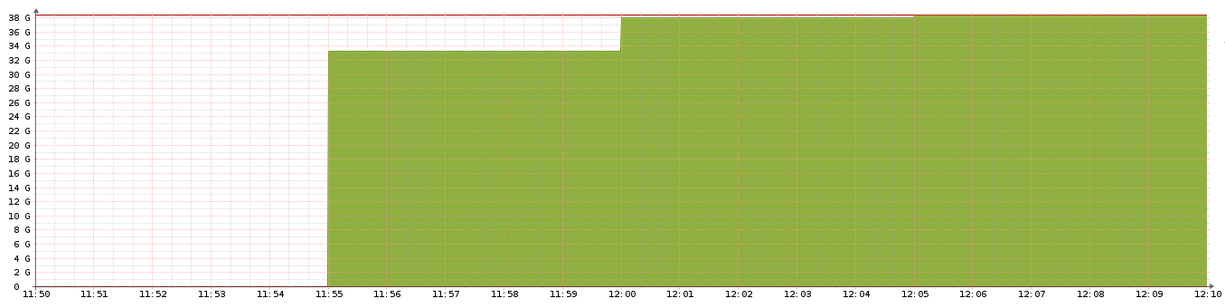
\includegraphics[scale=0.35]{images/pktgen_link_usage.png}
%  \caption{Pktgen link usage for 400 byte packets (generated bandwidth at time x, graph displays an average of used bandwidth over 5 minutes}
%  \label{fig:pktgenlink}
%\end{figure}

%\begin{figure}[H]
%  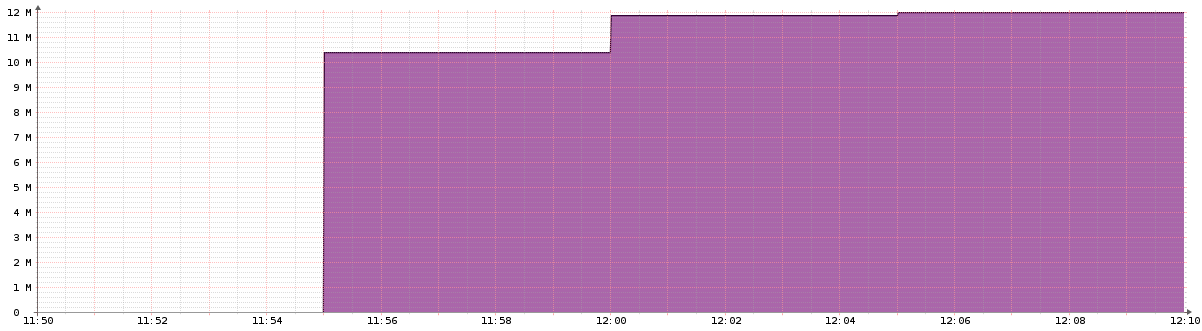
\includegraphics[scale=0.35]{images/pktgen_pps.png}
%  \caption{Pktgen packets per second for 400 byte packets (generated packets per second at time x, graph displays the average transported pps over 5 minutes}
%  \label{fig:pktgenpps}
%\end{figure}

\subsection{MoonGen}
MoonGen offers benchmark scripts to determine the machines capabilities. 
The benchmark script used for the tests can be found in appendix \ref{app:benchmark}. 
A single machine (B) is connected to the switch using two 40Gb/s ports at 2 separate cards (similar to the setup of the WARP test), both connected to switch S (one NIC for the server part and the other for the clients part of the benchmark). Sending UDP traffic with a size of 1500 bytes resulted in a maximum of 24 Gb/s. When the smallest possible Ethernet packets of 64 bytes are sent over the line a maximum of 15Mpps is reached. When TCP is used on the same machine (B) connected to the switch using two interfaces, a maximum of 10Gb/s was reached. These low values did not make MoonGen interesting enough since Pktgen is capable of reaching hardware limits. 

\subsection{WARP}\label{sub:warp}
In order to get to know the capabilities of DPDK in combination with WARP on top of the hardware in the experimentation environment a benchmark was run on server B.
A machine running WARP as a client needs a service to respond to SYN packets, otherwise sessions are not opened and there will not be any traffic flowing between client and server. 
Appendix \ref{app:benchmark} displays the benchmark script used for this test.
For this benchmark the server B  will be acting as the client and as the destination for the traffic, both client and destination are using a dedicated NIC. 
An extra Intel XL710 card is added to machine B since the XL710 card (which is a NIC providing two ports) can not utilize both ports in one slot at their full capacity\cite{intellinuxguidxl710}.
The second port on the card is designed as a fail-over interface. 
Port A from card one and two are connected to switch S. 
Traffic is generated from port A of NIC 1 to port A of NIC 2.
All of the machine's CPUs and memory will be dedicated to this test. 
The benchmark first does the tests for raw TCP, where after it will perform the tests using HTTP.

The client side of the benchmark attempted to open 4 million session although not all of the session succeed.
The amount of sessions per second, packets per second and the used bandwidth is registered along with the time spent until all sessions are tried. 
When a TCP session is opened between client and server, the tests will request a file or send a raw TCP packet.
The raw TCP reply is a TCP packet, for the HTTP file request a padded 200-OK message is returned. 
The goal for this test is to find the capabilities of the server while it is running WARP therefore the guidelines for bandwidth testing regarding runtime from RFC2544 are not applicable. 

The first test is raw TCP. As seen in figure \ref{fig:rawtcpsession} about one million sessions per second are tempted to open by the client.
When the packet size goes up the amount of sessions per second drops slightly.
The succeeded sessions use up some of the link's total capacity as is displayed in figure \ref{fig:rawtcplink}.
This means that the sessions that succeed are capable of filling 50 \% of the link capacity.  

\begin{figure}[H]
  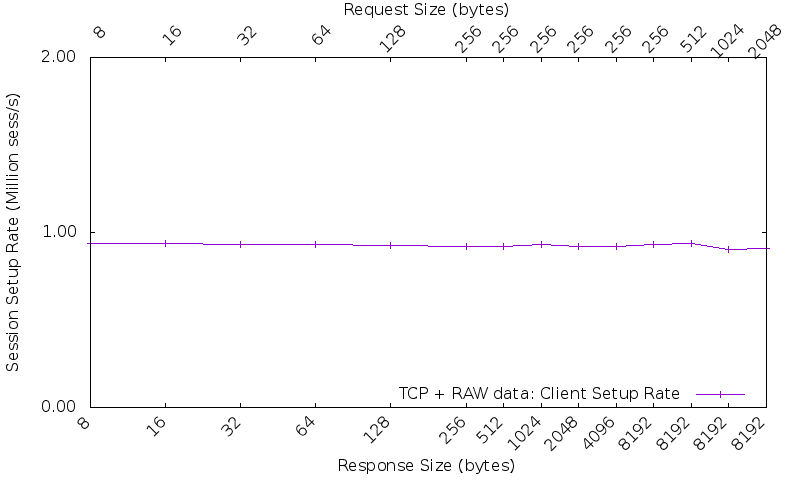
\includegraphics[scale=0.6]{images/raw_setup.png}
  \caption{Amount of requested session per second from the client to the server for raw TCP (amount of requested sessions versus the request(Rx) and respond(Tx) size)}
  \label{fig:rawtcpsession}
\end{figure}

\begin{figure}[H]
  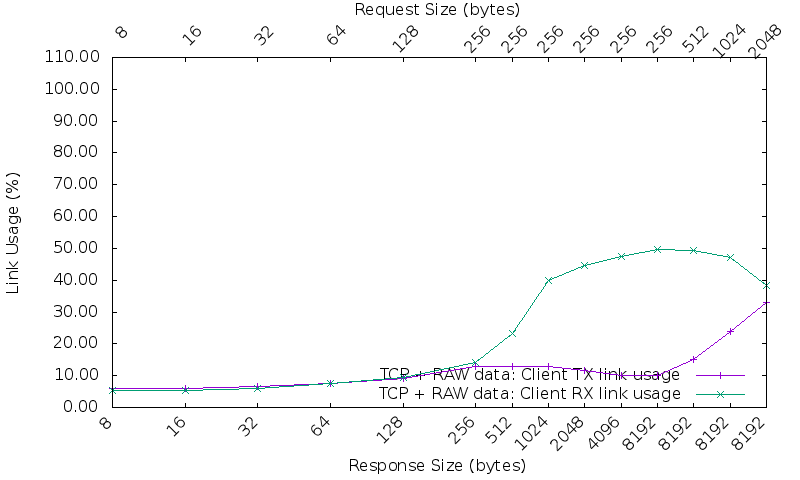
\includegraphics[scale=0.6]{images/raw_link_usage.png}
  \caption{Link usage for raw TCP (percentage of link usage versus the request(Rx) and response(Tx) size)}
  \label{fig:rawtcplink}
\end{figure}

The second test contains a HTTP file request. The server responds with a 200-(OK) message using a configured file size.
The server is able to generate around one million sessions per second as seen in figure \ref{fig:httpsession} but not all of the sessions were answered in time.
Figure \ref{fig:httplink} shows the bandwidth usage for HTTP traffic for the established sessions is at most 50\%. 

%The multiplication of the generated amount of session per second and the packet size will be more then the link's capacity. The graphs in figures \ref{fig:httpsession} and \ref{fig:rawtcpsession} displays the sessions per second the client tried to open. Successful sessions are not registered during the benchmark.    

\begin{figure}[H]
  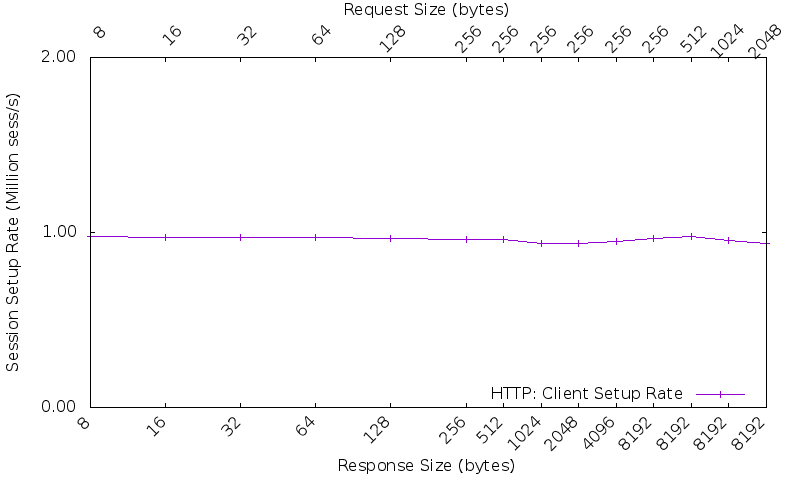
\includegraphics[scale=0.6]{images/http_setup.png}
  \caption{Amount of requested sessions per second from the client to the server for HTTP (amount of requested sessions versus the request(Rx) and respond(Tx) size)}
  \label{fig:httpsession}
\end{figure}

\begin{figure}[H]
  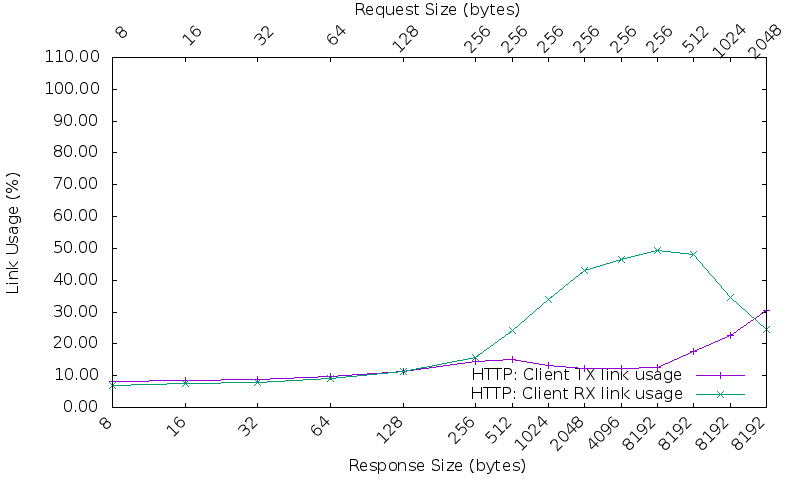
\includegraphics[scale=0.6]{images/http_link_usage.png}
  \caption{link usage for established sessions at HTTP  (percentage of link usage versus the request(Rx) and response(Tx) size)}
  \label{fig:httplink}
\end{figure}

From the figures we can see WARP is capable of generating 1 million sessions per second for both raw TCP and HTTP traffic. 
It can fill up half of the link capacity when large packets are generated.

WARP is capable of generating 1 million sessions per second for raw TCP and HTTP traffic towards a destination, when the packet size increases it can generate 20Gb/s of application layer data.
For stateful devices in a path to a server, the amount of sessions can be problematic. Overload behavior is expected from stateful devices in a path when WARP is used for limitation testing.  
This makes WARP useful for application level testing purposes. 

